\documentclass{article}

\usepackage{graphicx}
\usepackage{color}

\definecolor{pblue}{rgb}{0.13,0.13,1}
\definecolor{pgreen}{rgb}{0,0.5,0}
\definecolor{pred}{rgb}{0.9,0,0}
\definecolor{pgrey}{rgb}{0.46,0.45,0.48}

\usepackage{listings}
\lstset{language=Java,
  showspaces=false,
  showtabs=false,
  breaklines=true,
  showstringspaces=false,
  breakatwhitespace=true,
  commentstyle=\color{pgreen},
  keywordstyle=\color{pblue},
  stringstyle=\color{pred},
  basicstyle=\ttfamily,
  moredelim=[il][\textcolor{pgrey}]{$ $},
  moredelim=[is][\textcolor{pgrey}]{\%\%}{\%\%}
}

\begin{document}

\begin{titlepage}
   \vspace*{\stretch{1.0}}
   \begin{center}
      \Large\textbf{Project Manual}\\
      \large\textit{Group Echo}
   \end{center}
   \vspace*{\stretch{2.0}}
\end{titlepage}

\tableofcontents

\newpage

\section{Completed Requirements}
This section contains a list of completed requirements and for some requirements how the fulfillment was achieved.

\begin{itemize}
\item Contract
\begin{itemize}
\item CN1 - completed - The buttons for deletion and saving of a changed contract are disabled, when the contract is not in status PREPARED and therefore changes are made impossible at that point. A change was made, as Creation is possible for all university staff members, this is specified in the problems section of the manual under "Role-based access control"
\item CN2 - completed
\item CN3 - completed
\item CN4 - completed
\item CN4a - completed
\item CN4b - completed
\item CN4c - completed
\item CN4d - completed
\item CN4e - completed through the usage of a library called JollyDays. The federal state is saved by contract and the calculation of the public holidays is done based upon that setting.
\item CN5 - completed 
\item CN6 - completed by disabling the save button if the chosen contract is not in PREPARED.
\item CN6a - completed by only making month and year choosable in the datepicker and setting the day to the first/last of the month.
\item CN7 - completed
\item CN8 - completed
\item CN9 - completed by disabling the button if the given condition does not apply.
\item CN10 - completed by saving it in a column of the contract table.
\item CN11 - completed through a modal, which pops up and informs the user, who then may chose to continue or cease the action.
\item CN12 - completed
\end{itemize}
\item Timesheet
\begin{itemize}
\item TS1 completed - upon the start of a contract all timesheets are created depending on the frequency set in the contract and for the entire timespan between start and end of the contract.
\item TS2 completed - once a timesheet is signed by the employee it gets moved to the 'waiting' sections of timesheets in the timesheet management of the employee. There it can be viewed but not changed.
\item TS3 open
\item TS4 - completed
\item TS5 - completed
\item TS6 - completed
\item TS7 - completed - in the time sheet management section of the webapp.
\item TS8 - completed
\item TS9 - completed - see TS2
\end{itemize}
\item Signatures
\begin{itemize}
\item SG1 - completed
\item SG1a - completed
\item SG2 - completed
\item SG3 - completed
\item SG4 - missed
\end{itemize}
\item Reminders
\begin{itemize}
\item Reminders are modelled as an own entity, which eases collecting them for a given person. They are created either by a scheduled job or directly, when the state of a timesheet gets changed by a user. Old reminders, which do not match the timesheetstatus get deleted in the process.
\item RE1 - completed - on every last day of a week and month a scheduled job runs at midnight and creates reminders for timesheets, which are still IN PROGRESS.
\item RE2 - completed
\item RE3 - completed
\item RE4 - completed - all existing reminders get sent daily
\item RE5 - completed - all reminders for a person get collected in a single text and then send in a single mail to the person
\end{itemize}
\item Archiving
\begin{itemize}
\item AR1 - completed
\item AR2 - completed - archived timesheets enter the 'inactive' section in timesheet management, where they can be viewed but not changed
\item AR3 - completed - a scheduled job runs every night and deletes all timesheets, which have exceeded their archive duration. Contracts, which do not have any timesheets and are not in status PREPARED (the timesheets of such contracts are not created yet) are deleted.
\item AR4 - completed - upon contract creation an archive duration in months can be chosen and is stored in a column.
\end{itemize}
\item Access Control
\begin{itemize}
\item src/main/java/echo/security contains security handlers, which are used to check whether a certain permission shall be granted or not to a user.
\item AC1 - completed via a connection to the universities LDAP directory. If unauthenticated users try to access a page other than the login page they are redirected to the login page.
\item AC2 - completed via the LDAP connection.Such roles can be viewed in the person management.
\item AC3 - completed. Only data, which the user is affiliated with is loaded and checks are performed, whether a user can change/delete data. 
\end{itemize}
\item User interface
\begin{itemize}
\item UI1 - completed
\item UI2 - completed with the BootsFaces library.
\item UI3 - completed
\item UI4 - completed with the BootsFaces library.
\end{itemize}
\item Internationalization
\begin{itemize}
\item IN1 - completed. The user can switch the language under "profile". The language is then stored in a PersonConfig. The page content is then loaded from property files for the specified language, which defaults to english.
\item IN2 - completed
\item IN3 - completed. German and English are available.
\item IN4 - completed
\item IN5 - completed
\item IN6 - completed. The messages of the Reminders can be found in ReminderMessages. They are stored in HashMaps, which have the language in ISO 639 code as a key and therefore easily extensible. The messages are always loaded for the current locale of the user.
\end{itemize}
\item Software Architecture
\begin{itemize}
\item SA1 - completed
\item SA2 - completed. It contains three modules - core, ejb and web.
\item SA3 - completed. Only JollyDays was used as a third-party library for holiday day calculation. Its usage was negotiated after a lab session.
\item SA4 - completed with the usage of JavaDB.
\item SA5 - completed in chapter 2.
\item SA6 - completed
\end{itemize}
\item Project manual
\begin{itemize}
\item PM1 - completed, can be found in GitLab.
\item PM2 - completed with this list :)
\item PM3 - completed in Chapter 3.
\item PM4 - completed in this list.
\item PM5 - missed
\end{itemize}
\end{itemize}
\newpage
\section{Architectural decisions}

\begin{figure}[h]
\caption{The directory tree of the three used modules.}
\centering
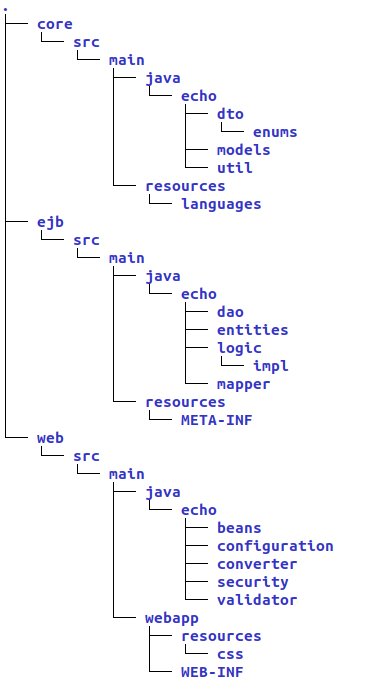
\includegraphics[width=200px]{structure}
\end{figure}
The source code is divided into three modules - core, ejb and web. The modules contentn bundles artifacts of a certain semantic domain within the system. The web module contains application logic and presentation layer and the ejb module contains business logic and data layer. The core module contains artifacts, which are used throughout the entire system, i.e. in the web and the ejb module. Inside the web module there are the webapp folder containing the templates and css and the java folder. Configuration holds logic to assign urls to .xhtml pages, beans the Backing Beans, converter classes for object conversion, validator validation classes and security the SecurityHandlers, which will be explained in the latter part of the manual. The ejb module is made up of access objects in dao, entities, business logic in logic and mappers in the mapper package, which provide mapping between dtos and entities. They are furtherly explained in the latter parts, as well. In the third module, the core module, there are Data Transfer Objects in dto, models, which are non-persistent, and util classes. Furthermore the core module holds the i18n language property files in the resource folder.\\
The systems architecture itself conforms to the layered architecture, which is outlined in the relevant documents. 
\subsection{Reminders}
\begin{figure}[h]
\caption{A small domain model, which shows the Reminder ecosystem of the TSS. Information not related to Reminders is left out for brevity.}
\centering
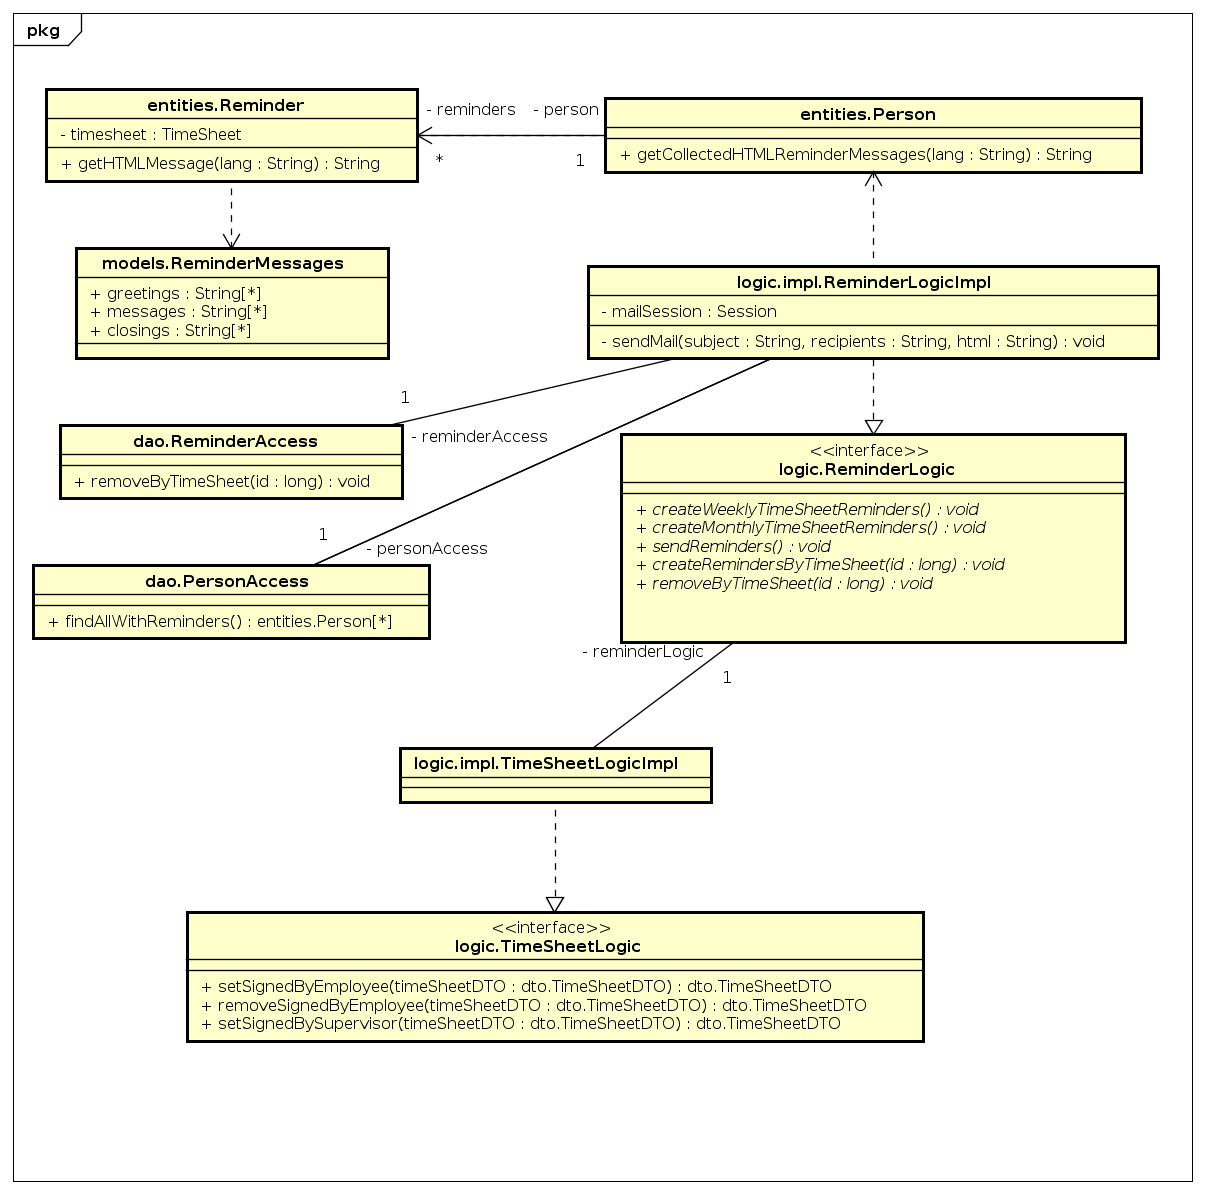
\includegraphics[width=\textwidth]{reminder_ecosystem}
\end{figure}
The Reminder ecosystem can be thought of as a subsystem of the TSS. \\ When realizing Reminders, the goal was to have an extensible solution, which is closed off to the end user and acts automatically depending on the status of a TimeSheet and eases collection of all Reminders for a user.\\
Therefore Reminders are modeled as an own entity and are associated with a TimeSheet and a Person. They are created automatically on the last day of week/month, in case a timesheet is still IN PROGRESS, and upon state changes to SIGNED BY EMPLOYEE and SIGNED BY SUPERVISOR, where now outdated ones also get deleted. Once the timesheet is ARCHIVED all reminders associated with it are deleted. Remindermails are sent via a scheduled job in the ReminderLogicImpl, which runs everyday. Every mail consists of a collection of all Reminders of the Person. \\ ReminderMessages contains HashMaps with the messages. They have the TimeSheetStatus and language in ISO 639 code as a key and can also easily be extended, e.g. by a new language, by adding an entry in the HashMaps. No changes elsewhere are necessary, which was an important design decision. Furthermore the status of the Reminders timesheet dictates the message, which therefore was not stored explicitly in the Reminder entity to hold memory consumption low.

\newpage

\subsection{Security}
\begin{figure}[h]
\caption{The abstract classes AbstractSecurityEvaluator and AbstractWebSecurityHandler.}
\centering
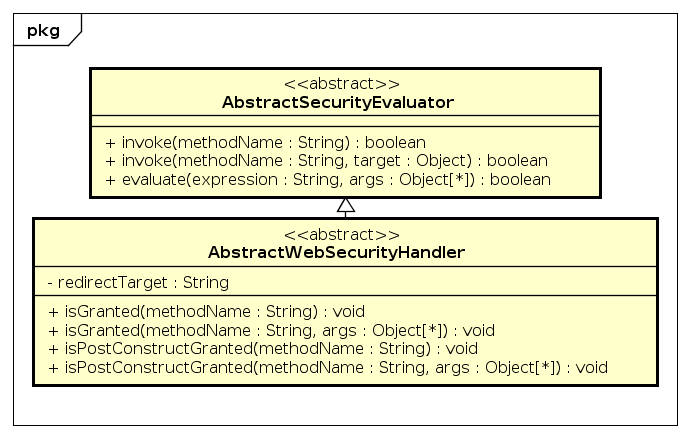
\includegraphics[width=\textwidth]{security_handler}
\end{figure}
To ensure security in the system, we opted to find a generic solution, which applied to different domains across the system such as authentication or ensuring, that an employee has the necessary roles within a contract to perform a certain operation. This was realized with the AbstractWebSecurityHandler and the AbstractSecurityEvaluator contained in web/src/main/java/echo/security.\\
The class AbstractWebSecurityHandler offers methods to check, whether a certain right is granted and can easily be extended to apply to different domains. The ContractWebSecurityHandler class for example contains methods to check all the roles in a contract and the LoggedInWebSecurityHandler offers ways of checking, whether a user is authenticated within the system, i.e. is logged in. \\
Additional important characteristic we opted for in the WebSecurityHandlers are ease-of-use and maintainability. This was achieved by having a uniform usage across the Handlers as is defined in the AbstractWebSecurityHandler. The Handlers can easily be injected into other EJBs. The code fragment from the TimeSheetBean, which backs the timesheet management page, below is supposed to illustrate its usage.
In the init() method it is firstly checked, whether the currently logged-in person is allowed to view the page. If this is not the case, the user is redirected to the SecurityHandlers redirectTarget, which defaults to the login page.\\
The onSelect method models the behaviour, when a contract is selected on the page. To enforce security by design only the contracts a person is associated with, i.e. has a role in, are loaded as is done in getAllContracts(). But incase a user was to fiddle with the url to try to gain access to contracts he has no role in, the check in onSelect would prevent him from doing so. 
\begin{lstlisting}
@EJB
private ContractWebSecurityHandler contractWebSecurityHandler;
@EJB
private LoggedInWebSecurityHandler loggedInWebSecurityHandler;
private ContractDTO selectedContract;
private PersonDTO sessionPerson;

@PostConstruct
public void init() {
	loggedInWebSecurityHandler.isPostConstructGranted(
		"#isAuthenticated($null)"
		)
    sessionCache.getSessionPerson().ifPresent(personDTO -> sessionPerson = personDTO);
}

public void onSelect(ContractDTO selectedContract) {
	contractWebSecurityHandler.isGranted("
		#hasRoleInContract($0)",
		selectedContract
		);
    this.selectedContract = selectedContract;
}

public List<ContractDTO> getAllContracts() {
	List<ContractDTO> relatedContracts = new ArrayList<>();

    if (sessionPerson != null) {
    	relatedContracts = timeSheetLogic.getRelatedContractsForPerson(sessionPerson);
    }
    
	return relatedContracts;
}

\end{lstlisting}
\newpage

\subsubsection{The AbstractSecurityEvaluator and its DSL}

The lines \begin{lstlisting}
loggedInWebSecurityHandler.isPostConstructGranted(
		"#isAuthenticated($null)"
		)
\end{lstlisting}
and 
\begin{lstlisting}
contractWebSecurityHandler.isGranted("
		#hasRoleInContract($0)",
		selectedContract
		);
\end{lstlisting}
show how the SecurityHandlers can be used to check authorization and rights with expressions. This is facilitated with a small DSL, which is based on logical expressions, implemented in the AbstractSecurityEvaluator. It enables users to check the return value of a certain method, which is indicated by the \#, optionally also with parameters, indicated by a \$ followed by the index of the argument. The selectedContract in the second listing for example would be used as an argument of the method hasRoleInContract, which is invoked via reflection. Additionally the expression handed to isGranted and isPostConstructGranted can contain composite expressions chained together with logical operators such as $\Vert$ or $\&\&$.
\newpage

\subsection{Mapper}
\begin{figure}[h]
\caption{The SimpleMapper class in src/main/java/echo/mapper.}
\centering
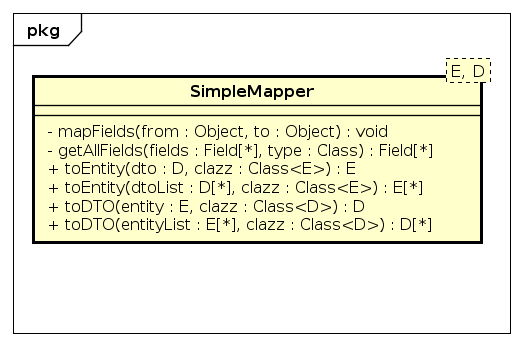
\includegraphics[width=\textwidth]{mapper}
\end{figure}
To enforce the architectural constraints regarding echo.entities, DTOs and their domains we also opted for a generic approach, which is easy to use and has a clearly defined usage pattern. The SimpleMapper class offers methods to map echo.entities to DTOs and vice versa, therefore easing the constant switching between the different objects and providing a uniform usage.\\
The SimpleMapper itself only offers mapping of non-@Entity relations and is extended multiple times in src/main/java/echo/mapper to provide mapping of Entities with non-primitive associations.

\section{Problems during development}
\subsection{Security}
While the majority of development work ran smoothly, setting up the Security was problematic. We planned to use Spring Security as a framework and more specifically the provided annotations to secure Business and Application Logic. This was problematic, as we had already implemented the logic behind the Login and authentication from the LDAP directory ourselves. Spring Security however builds upon the Login logic contained in the Spring framework. Therefore we would have either had to rebuild the Login logic with Spring or build an approach ourselves. As rebuilding would have taken too long and using the Spring framework this extensively, which would have been required in order to use Spring Security efficiently, would surely not have been the aim of the course, we opted for an own implementation, which has already been described furtherly in chapter 2.
\subsection{Role-based access control}
The implementation of the role-based access control was smoothly implemented within the contract, where we permitted actions according to the role of the contract as was specified in the requirements. On system level however it was in parts not clear to us, how to implement the specific roles as some would have resulted in a chicken or the egg dilemma. If for example only secretaries and delegates were allowed to create contracts, at which point would they become secretaries or delegates? If that was only the case once they had such role in any contract, that could have been a problem. Therefore we set up the person management, which is only available to administrators in a way, that staff members can be assigned roles prior to being associated with any contract within the system. As this creates the next chicken or the egg dilemma, the first Administrator has to be put into the database manually. Contracts can also be created by any staff member of the university, as the requirements did not specify the behaviour outside of contracts.
\newpage

\end{document}